\documentclass[fontset=windows]{article}
\usepackage[margin=1in]{geometry}%设置边距,符合Word设定
\usepackage[UTF8]{ctex}
\usepackage{setspace}
\usepackage{amsmath}
\usepackage{amssymb}
\numberwithin{figure}{section}
\usepackage{array}
\usepackage{lipsum}
\usepackage{float}
\usepackage{graphicx}%插入图片
\usepackage[dvipsnames]{xcolor}
\usepackage{authblk}
\usepackage{listings,matlab-prettifier}
\lstset{
	language=Matlab, % 设置代码语言为Matlab
    basicstyle=\ttfamily, % 设置字体为等宽字体
    numbers=left, % 行号在左边显示
    numberstyle=\tiny, % 设置行号字体大小
    stepnumber=1, % 行号递增步长
    numbersep=5pt, % 行号到代码的距离
    backgroundcolor=\color{gray!10}, % 设置代码的背景颜色
    showspaces=false,
    showstringspaces=false,
    showtabs=false,
    frame=single, % 设置代码框
    rulecolor=\color{black},
    tabsize=2,
    breaklines=true,
    breakatwhitespace=true,
    title=\lstname,
	keywordstyle=\bfseries\color{NavyBlue},
	morekeywords={var,};
	emphstyle=\bfseries\color{Rhodamine}, % 强调词样式设置
    commentstyle=\itshape\color{black!50!white}, % 设置注释样式,斜体,浅灰色
    stringstyle=\bfseries\color{PineGreen!90!black}, % 设置字符串样式
	columns=flexible,}
\graphicspath{{Figures7/}}%文章所用图片在当前目录下的 Figures目录

\usepackage{hyperref} % 对目录生成链接,注:该宏包可能与其他宏包冲突,故放在所有引用的宏包之后
\hypersetup{colorlinks = true,  % 将链接文字带颜色
	linkcolor=black, % 将链接文字黑色
	bookmarksopen = true, % 展开书签
	bookmarksnumbered = true, % 书签带章节编号
	} % 作者
\bibliographystyle{plain}% 参考文献引用格式

\renewcommand{\contentsname}{\centerline{目录}} %经过设置word格式后,将目录标题居中

\title{\heiti\zihao{2} 《统计信号处理》第七教学单元研讨题}
\author{杨 鼎,韦可雷,高司博,高涵博}
\date{}

\begin{document}
\maketitle
\thispagestyle{empty}

%\begin{abstract}
%	\lipsum[2]
%\end{abstract}

%\tableofcontents
%\setcounter{page}{0}
%\newpage

\section{研讨题1}
考虑二元假设问题

\begin{align*}
    \begin{matrix}
        \mathcal{H}_0: & z[k]=n[k]      \\
        \mathcal{H}_1: & z[k]=s[k]+n[k]
    \end{matrix}\quad k=0,1,\ldots,N-1
\end{align*}
噪声是服从\(n(k)\sim \mathcal{N}(0,\sigma^2)\)的WGN。

\subsection*{(1)若\(s[k]=A,A\sim \mathcal{N}(0,\sigma^2_A)\)且与噪声独立,\(\sigma^2_A\)已知,求解NP判决式。}

参照例5.1,由于信号服从\(A\sim \mathcal{N}(0,\sigma^2_A)\)的WGN,所以在\(\mathcal{H}_0\)条件下,\(\mathbf{z}\sim \mathcal{N}(\mathbf{0},\sigma^2\mathbf{I})\),在\(\mathcal{H}_1\)条件下,\(\mathbf{z}\sim \mathcal{N}(\mathbf{0},(\sigma^2+\sigma^2_A)\mathbf{I})\),

根据NP准则,如果似然比超过门限
\begin{align*}
    L(\mathbf{z})=\frac{p(\mathbf{z};\mathcal{H}_1)}{p(\mathbf{z};\mathcal{H}_0)}>\gamma
\end{align*}
则NP检测器判\(\mathcal{H}_1\)。
其中
\begin{align*}
    p(\mathbf{z};\mathcal{H}_1)
     & =\frac{1}{[2\pi (\sigma_A^2+\sigma^2)]^{N/2}}\exp
    \left[-\frac{1}{2(\sigma^2_s+\sigma^2)}\sum_{n=0}^{N-1}z^2[n] \right] \\
    p(\mathbf{z};\mathcal{H}_0)
     & =\frac{1}{(2\pi\sigma^2)^{N/2}}\exp
    \left[-\frac{1}{2\sigma^2}\sum_{n=0}^{N-1}z^2[n] \right]
\end{align*}
对数似然比可以求得
\begin{align*}
    \ln L(\mathbf{z})
     & =\frac{N}{2}\ln(\frac{\sigma^2}{\sigma^2+\sigma^2_A})-
    \frac{1}{2}(\frac{1}{\sigma^2_s+\sigma^2}-\frac{1}{\sigma^2})\sum_{n=0}^{N-1}z^2[n] \\
     & =\frac{N}{2}\ln(\frac{\sigma^2}{\sigma^2+\sigma^2_A})
    +\frac{1}{2}\frac{\sigma^2_A}{(\sigma^2_A+\sigma^2)\sigma^2}\sum_{n=0}^{N-1}z^2[n]
\end{align*}
如果
\begin{align*}
    T(\mathbf{z})=\sum_{n=0}^{N-1}z^2[n]>2\sigma^2(1+\frac{\sigma^2}{\sigma^2_A})\left[\ln \gamma+\frac{N}{2}\ln(1+\frac{\sigma^2_A}{\sigma^2})\right]=\gamma^{\prime}
\end{align*}
则\(\mathcal{H}_1\)成立。

\subsection*{(2)若\(s[k]\sim Ar^k(0<r<1),A\sim \mathcal{N}(0,\sigma^2_A)\)且与噪声独立,\(\sigma^2_A\)已知,求解NP判决式。}

若\(s[k]\sim Ar^k(0<r<1)\),假设可以重写为线性模型
\begin{align*}
    \mathcal{H}_0 & :\mathbf{z}=\mathbf{n}             \\
    \mathcal{H}_1 & :\mathbf{z}=\mathbf{H}A+\mathbf{n}
\end{align*}
其中
\begin{align*}
    \mathbf{z}=
     & \begin{bmatrix}
           z[0] & z[1] & \cdots & z[N-1]
       \end{bmatrix}^T \\
    \mathbf{n}=
     & \begin{bmatrix}
           n[0] & n[1] & \cdots & n[N-1]
       \end{bmatrix}^T \\
    \mathbf{H}=
     & \begin{bmatrix}
           0 & r & \cdots & r^k
       \end{bmatrix}^T
\end{align*}
由于\(A\sim \mathcal{N}(0,\sigma^2_A)\)且与噪声独立,所以
\begin{align*}
    \mathbf{z}\sim\left\{
    \begin{matrix}
        \mathcal{N}(\mathbf{0},\sigma^2\mathbf{I})                         & ,\mathcal{H}_0 \\
        \mathcal{N}(\mathbf{0},\sigma^2_A\mathbf{HH}^T+\sigma^2\mathbf{I}) & ,\mathcal{H}_1
    \end{matrix}
    \right.
\end{align*}

类似第\(\mathbf{(1)}\)问,根据NP准则,如果似然比
\begin{align*}
    L(\mathbf{z})=\frac{p(\mathbf{z};\mathcal{H}_1)}{p(\mathbf{z};\mathcal{H}_0)}>\gamma
\end{align*}
则NP检测器判\(\mathcal{H}_1\)。其中
\begin{align*}
    p(\mathbf{z};\mathcal{H}_1)
     & =\frac{1}{(2\pi)^{N/2} \det^{1/2}(\sigma^2_A\mathbf{HH}^T+\sigma^2\mathbf{I})}
    \exp\left[-\frac{1}{2}\mathbf{z}^T(\sigma^2_A\mathbf{HH}^T+\sigma^2\mathbf{I})^{-1}\mathbf{z} \right] \\
    p(\mathbf{z};\mathcal{H}_0)
     & =\frac{1}{(2\pi\sigma^2)^{N/2}}\exp
    \left(-\frac{1}{2\sigma^2}\mathbf{z}^T\mathbf{z} \right)
\end{align*}
对数似然比可以求得
\begin{align*}
    \ln L(\mathbf{z})
     & =-N\ln(\sigma)+\frac{1}{2}\ln \det(\sigma^2_A\mathbf{HH}^T+\sigma^2\mathbf{I})
    -\frac{1}{2}\mathbf{z}^T(\sigma^2_A\mathbf{HH}^T+\sigma^2\mathbf{I})^{-1}\mathbf{z}
    +\frac{\mathbf{z}^T\mathbf{z}}{{2\sigma^2}}                                       \\
     & =-N\ln(\sigma)+\frac{1}{2}\ln(\sigma^2+\sigma^2_A\mathbf{HH}^T)
    +\frac{1}{2}\mathbf{z}^T\left[-(\sigma^2_A\mathbf{HH}^T+\sigma^2\mathbf{I})^{-1}+\frac{1}{\sigma^2}\mathbf{I}\right]\mathbf{z}
\end{align*}
利用矩阵求逆引理
\begin{align*}
    (\mathbf{A}+\mathbf{BCD})^{-1}=A^{-1}-\mathbf{A}^{-1}\mathbf{B}(\mathbf{DA}^{-1}\mathbf{B}+\mathbf{C}^{-1})^{-1}\mathbf{DA}^{-1}
\end{align*}
令\(\mathbf{A}=\sigma^2\mathbf{I},\mathbf{B}=\mathbf{H},\mathbf{D}=\mathbf{H}^T,\mathbf{C}=\sigma^2_A\mathbf{I}\),得到
\begin{align*}
    (\sigma^2_A\mathbf{HH}^T+\sigma^2\mathbf{I})^{-1}
     & =\frac{1}{\sigma^2}\mathbf{I}-
    \frac{1}{\sigma^2}\mathbf{IH}(\mathbf{H}^T\frac{1}{\sigma^2}\mathbf{IH}+\frac{1}{\sigma^2_A}\mathbf{I})^{-1}
    \mathbf{H}^T\frac{1}{\sigma^2}\mathbf{I}                                                                                                \\
     & =\frac{1}{\sigma^2}\mathbf{I}-\frac{\sigma^2_A\mathbf{H}^T\mathbf{H}}{\sigma^2(\sigma^2+\sigma^2_A\mathbf{H}^T\mathbf{H})}\mathbf{I} \\
     & =\frac{\mathbf{I}}{\sigma^2+\sigma^2_A\mathbf{H}^T\mathbf{H}}
\end{align*}
所以对数似然函数
\begin{align*}
    \ln L(\mathbf{z})
     & =-N\ln(\sigma)+\frac{1}{2}\ln(\sigma^2+\sigma^2_A\mathbf{HH}^T)
    +\frac{1}{2}(-\frac{1}{\sigma^2+\sigma^2_A\mathbf{H}^T\mathbf{H}}+\frac{1}{\sigma^2})\mathbf{z}^T\mathbf{z}        \\
     & =-N\ln(\sigma)+\frac{1}{2}\ln(\sigma^2+\sigma^2_A\mathbf{HH}^T)+
    \frac{\sigma^2_A\mathbf{H}^T\mathbf{H}}{\sigma^2(\sigma^2+\sigma^2_A\mathbf{H}^T\mathbf{H})}\mathbf{z}^T\mathbf{z} \\
     & >\ln \gamma
\end{align*}
时,判\(\mathcal{H}_1\)。

由于\(\sigma^2,\sigma^2_A\)均已知,可以整理为
\begin{align*}
    T(\mathbf{z}) & =\mathbf{z}^T\mathbf{z}                                                                       \\
                  & >\frac{\sigma^2(\sigma^2+\sigma^2_A\mathbf{H}^T\mathbf{H})}{\sigma^2_A\mathbf{H}^T\mathbf{H}}
    (\ln \gamma+N\ln (\sigma)-\frac{1}{2}\ln(\sigma^2+\sigma^2_A\mathbf{HH}^T))                                   \\
                  & =\gamma^{\prime\prime}
\end{align*}
则\(\mathcal{H}_1\)成立。其中\(\mathbf{H}^T\mathbf{H}=\sum_{k=0}^{N-1}r^{2k}=\frac{1-r^{2N}}{1-r^2}\)。


\subsection*{(3)若\(s[k]=A\cos(2\pi f_0 k+\phi )\),A已知但\(\phi\)未知,若检验统计量采用\(\sum_{k=0}^{N-1}z[k]A\cos(2\pi f_0 k)\),讨论大N情况下偏移系数及其与\(\phi\)的关系。}
假设\(\phi\)服从均匀分布,\(\phi\sim \mathcal{U}(0,2\pi)\),则\(E\left[\cos(\phi)\right]=E\left[\sin(\phi)\right]=0\)

\begin{align*}
    E(T;\mathcal{H}_1)
     & =E\left[\sum_{k=0}^{N-1}z[k]A\cos (2\pi f_0 k)\right]                                        \\
     & =E\left[\sum_{k=0}^{N-1}(s[k]+n[k])A\cos (2\pi f_0 k)\right]                                 \\
     & =E\left[\sum_{k=0}^{N-1}A^2\cos(2\pi f_0 k+\phi)\cos (2\pi f_0 k)\right]                     \\
     & =E\left\{\sum_{k=0}^{N-1}\frac{A^2}{2}\left[\cos(4\pi f_0 k+\phi)+\cos (\phi)\right]\right\} \\
     & =\frac{NA^2}{2}\cos(\phi)+E\left[\sum_{k=0}^{N-1}\frac{A^2}{2}\cos(4\pi f_0 k+\phi)\right]   \\
     & =\frac{NA^2}{2}\cos(\phi)
\end{align*}

\begin{align*}
    E(T;\mathcal{H}_0)
     & =E\left[\sum_{k=0}^{N-1}z[k]A\cos (2\pi f_0 k)\right] \\
     & =E\left[\sum_{k=0}^{N-1}n[k]A\cos (2\pi f_0 k)\right] \\
     & =0
\end{align*}
由于噪声\(n[k]\sim\mathcal{N}(0,\sigma^2)\)的WGN,所以\(E\left[n[k]n[l]\right]=\delta(k,l)\sigma^2\)
\begin{align*}
    Var(T;\mathcal{H}_0)
     & =E\left\{\left[\sum_{k=0}^{N-1}z[k]A\cos (2\pi f_0 k)\right]^2 \right\}-E^2\left[\sum_{k=0}^{N-1}z[k]A\cos (2\pi f_0 k)\right] \\
     & =A^2E\left[\sum_{k=0}^{N-1}\sum_{l=0}^{N-1}n[k]n[l]\cos (2\pi f_0 k)\cos (2\pi f_0 l)\right]                                   \\
     & =A^2\sigma^2\sum_{k=0}^{N-1}\cos^2 (2\pi f_0 k)                                                                                \\
     & =\frac{A^2\sigma^2}{2}\sum_{k=0}^{N-1}1+\cos (4\pi f_0 k)
\end{align*}
对于大的N值
\begin{align*}
    \frac{1}{N}\sum_{k=0}^{N-1}\cos k\alpha
     & =\frac{1}{N}Re\left(\sum_{k=0}^{N-1}\exp(jk\alpha)\right)                             \\
     & =\frac{1}{N}Re\left[\exp(j(N-1)\alpha/2)\frac{\sin(N\alpha/2)}{\sin(\alpha/2)}\right] \\
     & \approx \frac{\sin(N\alpha)}{2N\sin(\alpha/2)}
\end{align*}
所以
\begin{align*}
    Var(T;\mathcal{H}_0)
     & \approx \frac{A^2\sigma^2}{2}(N+\frac{\sin(N\alpha)}{2\sin(\alpha/2)}) \\
     & \approx\frac{NA^2\sigma^2}{2}
\end{align*}

偏移系数
\begin{align*}
    d^2
     & =\frac{\left[E(T;\mathcal{H}_1)-E(T;\mathcal{H}_0)\right]^2}{Var(T;\mathcal{H}_0)} \\
     & =\frac{NA^2}{2\sigma^2}\cos^2 \phi
\end{align*}
偏移系数与\(\phi\)有关,当\(\phi=0,\pi\)时,检测性能最佳,当\(\phi=\pi/2,3\pi/2\)时,检测性能最差。

这是由于检验统计量\(\sum_{k=0}^{N-1}z[k]A\cos(2\pi f_0 k)\)不能构成单一的充分统计量。

由于\(s[n]=A\cos (2\pi f_0 k+\phi)\),
\begin{align*}
    p(\mathbf{z};\mathcal{H}_1)
    =  \frac{1}{(2\pi \sigma^2)^{N/2}}
     & \exp\left\{-\frac{1}{2\sigma^2}\sum_{k=0}^{N-1}[z[n]-A\cos (2\pi f_0 k+\phi)]^2 \right\}                                                        \\
    =  \frac{1}{(2\pi \sigma^2)^{N/2}}
     & \exp\bigg\{-\frac{1}{2\sigma}\bigg[\sum_{k=0}^{N-1}z^2[n]-2A\left(\sum_{k=0}^{N-1}z[n]\cos2\pi f_0 k\right)\cos \phi                            \\
     & +2A\left(\sum_{k=0}^{N-1}z[n]\sin 2\pi f_0 k\right)\sin \phi\bigg] +\sum_{k=0}^{N-1}A^2\cos^2 (2\pi f_0 k +\phi)\bigg\}                         \\
    = \frac{1}{(2\pi \sigma^2)^{N/2}}
     & \exp\left\{-\frac{1}{2\sigma^2}\left[\sum_{k=0}^{N-1}A^2\cos(2\pi f_0 k+\phi)-2T_1(\mathbf{z})\cos\phi+2T_2(\mathbf{z})\sin \phi\right]\right\} \\
     & \cdot \exp\left[-\frac{1}{2\sigma^2}\sum_{k=0}^{N-1}z^2[n]\right]                                                                               \\
     & =g(T(\mathbf{z}),T_2(\mathbf{z}),\phi)\cdot h(\mathbf{z})
\end{align*}
其中
\begin{align*}\
    T_1(\mathbf{z}) & =\sum_{k=0}^{N-1}Az[n]\cos2\pi f_0 k \\
    T_2(\mathbf{z}) & =\sum_{k=0}^{N-1}Az[n]\sin2\pi f_0 k
\end{align*}

根据Neyman-Fisher因子分解定理,\(T_1(\mathbf{z})\)和\(T_2(\mathbf{z})\)共同构成充分统计量,单一的\(T_1(\mathbf{z})\)并没有包含进行NP假设检验的所有信息。

\section{研讨题2:雷达信号检测问题。}
考虑二元假设检验问题

\begin{align*}
    \begin{matrix}
        H_0: & z(k)=n(k)      \\
        H_1: & z(k)=s[k]+n(k)
    \end{matrix}\quad k=0,1,\cdots N-1
\end{align*}
其中噪声\(n(k)\)是服从\(n(k)\sim \mathcal{N}(0,\sigma^2)\)的WGN。

\subsection*{1、若\(s[k]=Ar^k,r\)已知且\(0<r<1,A\sim \mathcal{N}(0,\sigma^2_A),\sigma^2_A\)未知且与噪声A独立,求GLRT判决式}


\subsection*{(2)若\(s[k]\)是广义平稳随机过程,其功率谱密度
    \begin{align*}
        P_s(f;P_0)=\left\{
        \begin{matrix}
            2P_0 & 0\leqslant f\leqslant 1/4 \\
            0    & 1/4<f\leqslant1/2
        \end{matrix}\right.
    \end{align*}
    其中\(P_0\)未知,求GLRT判决式。}

\section{研讨题3}

高斯噪声中已知信号的分析与仿真,考虑二元假设
\begin{align*}
    \begin{matrix}
        H_0: & z(k)=n(k)      \\
        H_1: & z(k)=s[k]+n(k)
    \end{matrix}\quad k=0,1,\cdots N-1
\end{align*}

噪声是服从\(n(k)\sim \mathcal{N}(0,5)\)的WGN,信号为零均值高斯随机信号,协方差矩阵\([\mathbf{C}]_{ij}=c[i-j],j=0,1,\ldots,N-1\),其中\(c[k]=\frac{1}{1-0.9^2}0.9^{|k|}\),若\(N=100\),虚警概率设定为0.01,试通过计算机模拟分析检测门限及检测概率。

\section{研讨题4}

能量检测器的分析与仿真:考虑二元假设
\begin{align*}
    \begin{matrix}
        H_0: & z(k)=n(k)      \\
        H_1: & z(k)=s[k]+n(k)
    \end{matrix}\quad k=0,1,\cdots N-1
\end{align*}
噪声是服从\(n(k)\sim \mathcal{N}(0,\sigma^2)\)的WGN,\(\sigma^2\)已知。

\subsection*{(1)若\(s(k)\)是完全未知确定信号,假定\(\sigma^2=1,N=10\),虚警概率设定为0.01,分析检测门限,能得到检测概率吗?}

若\(s(k)\)是完全未知确定信号,则使用最大似然估计\(\hat{s}(k)=z(k)\),似然比为

\begin{align*}
    \Lambda(\mathbf{z})=\frac{p(\mathbf{z}|\hat{s}[0],\hat{s}[2],\ldots,\hat{s}[N-1],\mathcal{H}_1)}{p(\mathbf{z}|\mathcal{H}_0)}
\end{align*}
化简可以得到检测统计量与检测门限为能量检测器的形式:
\begin{align*}
    T(\mathbf{z})=\sum_{n=0}^{N-1}z^2[n]=\sum_{n=0}^{N-1}z[n]z[n]=\sum_{n=0}^{N-1}z[n]\hat{s}[n]>\gamma
\end{align*}
若要得到其检测性能,必须限定一个大前提,即大数据量,小信噪比的时候,近似有
\begin{align*}
    P_D\approx Q[Q^{-1}(P_F)-d^2]
\end{align*}
其中\(d^2=\frac{(\epsilon/\sigma^2)^2}{2N}\),\(\epsilon/\sigma^2\)为信噪比。

虚警概率为0.01的检测概率仿真图如下,其中第一张图是不限定信噪比的检测概率,考虑到检测性能前提,画出了信噪比低于0dB条件下的检测概率曲线,可以看出,检测概率较小。
\begin{figure}[H]
    \centering
    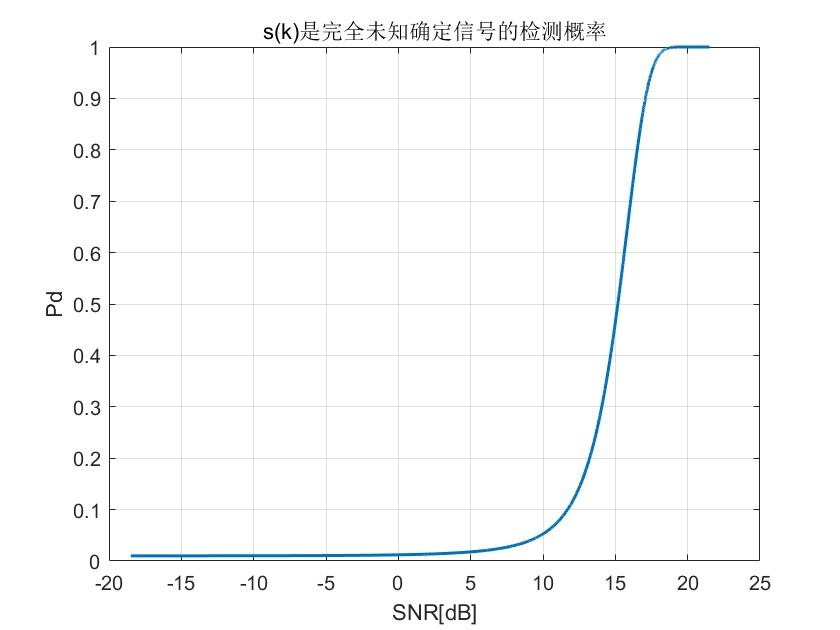
\includegraphics[scale=0.5]{fig4.1.jpg}
    \caption{\(s(k)\)是完全未知确定信号的检测概率}
    \label{4.1}
\end{figure}

\begin{figure}[H]
    \centering
    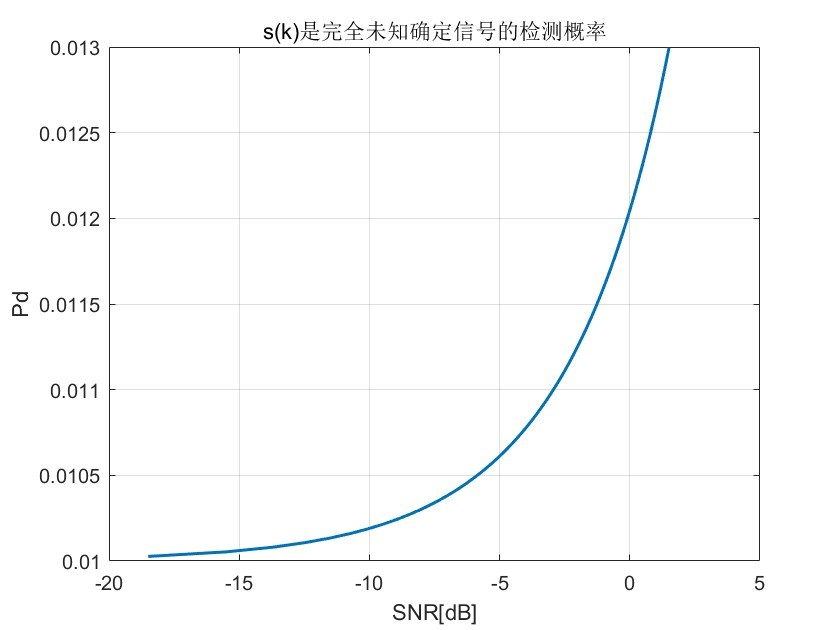
\includegraphics[scale=0.5]{fig4.2.jpg}
    \caption{\(s(k)\)是完全未知确定信号的检测概率}
    \label{4.2}
\end{figure}



\subsection*{(2)若\(s(k)\)是均值为零方差为\(\sigma^2_s\)的白高斯信号,假定\(\sigma^2=\sigma^2_s=1,N=100\),虚警概率设定为0.01,试分析检测门限及检测概率并仿真。}

若\(s(k)\)是均值为零,方差为\(\sigma^2_s=1\)的高斯白噪声,为典型的高斯白噪声的高斯白噪声随机信号检测,似然比为
\begin{align*}
    \Lambda(\mathbf{z})=\frac{p(\mathbf{z}|\mathcal{H}_1)}{p(\mathbf{z}|\mathcal{H}_0)}>\eta
\end{align*}
由此可以化简得到检验统计量与门限
\begin{align*}
    T(\mathbf{z})=\sum_{n=0}^{N-1}z^2[n]>\gamma
\end{align*}
与确定性信号不同的是,由于信号和噪声均分从高斯分布,则有
\begin{align*}
    \chi^2_N\sim\left\{
    \begin{matrix}
        \frac{T(\mathbf{z})}{\sigma^2}            & , \mathcal{H}_0 \\
        \frac{T(\mathbf{z})}{\sigma^2+\sigma^2_s} & , \mathcal{H}_1
    \end{matrix}
    \right.
\end{align*}
因此虚警概率与检测门限分别为
\begin{align*}
    P_F    & =Pr\{T(\mathbf{z})>\gamma|\mathcal{H}_0\}=Pr\left\{ \frac{T(\mathbf{z})}{\sigma^2}>\frac{\gamma^2}{\sigma^2}|\mathcal{H}_0\right\}=Q_{\chi^2_N}(\frac{\gamma}{\sigma^2}) \\
    \gamma & =\sigma^2Q^{-1}_{\chi^2_N}(P_F)
\end{align*}
检测概率为
\begin{align*}
    P_D
     & =Pr\left\{T(\mathbf{z})>\gamma|\mathcal{H}_1 \right\}                                                         \\
     & =Pr\left\{\frac{T(\mathbf{z})}{\sigma^2+\sigma^2_s}<\frac{\gamma}{\sigma^2+\sigma^2_s} |\mathcal{H}_1\right\} \\
     & =Q_{\chi^2_N}\left(\frac{\gamma}{\sigma^2+\sigma^2_s}\right)                                                  \\
     & =Q_{\chi^2_N}\left(\frac{\sigma^2Q^{-1}_{\chi^2_N}(P_F)}{\sigma^2+\sigma^2_s}\right)                          \\
     & =Q_{\chi^2_N}\left(\frac{Q^{-1}_{\chi^2_N}(P_F)}{\sigma^2_s/\sigma^2+1}\right)
\end{align*}
由卡方右尾函数性质可知,当信噪比\(\sigma^2_s/\sigma^2\)增加,检测概率增减,限定虚警概率为0.01条件下,仿真检测性能曲线如下

\begin{figure}[H]
    \centering
    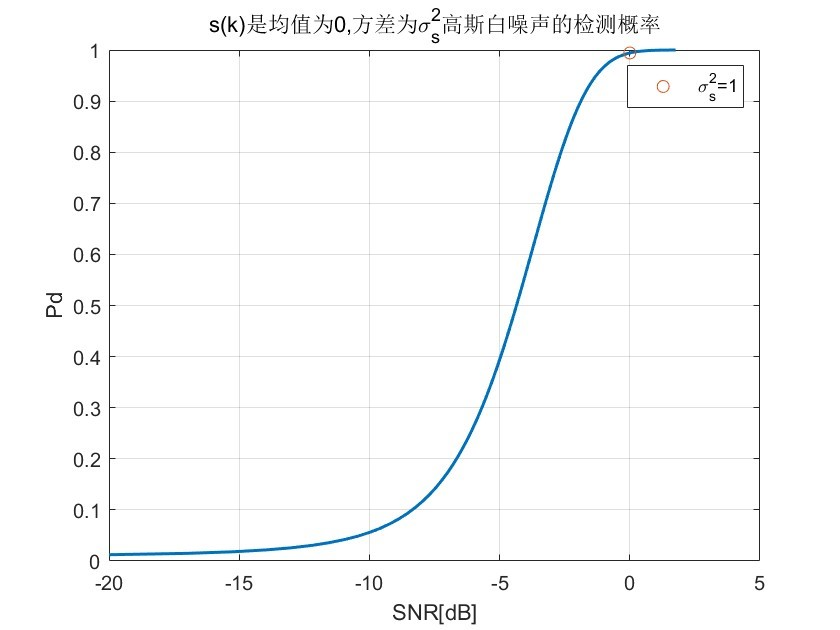
\includegraphics[scale=0.6]{fig4.3.jpg}
    \caption{\(s(k)\)是均值为0,方差为\(\sigma^2_s\)高斯白噪声的检测概率}
    \label{4.3}
\end{figure}

其中当\(\sigma^2=\sigma^2_s=1\)时,门限为135.8067,检测概率\(P_D=99.42\%\)

\bibliography{books}
\end{document}